\documentclass[]{extarticle}

\usepackage[]{fancyhdr}
\usepackage[french]{babel}
\usepackage[svgnames, table]{xcolor}
\usepackage[]{geometry}
\usepackage[]{graphicx}
\usepackage[]{setspace}

\pagestyle{fancy}
\fancyhead[L]{The Believer's Quest}
\geometry{hmargin=3cm,vmargin=2.5cm}

\begin{document}
\begin{spacing}{1.25}

\textsc{ }\\
\textsc{ }\\
\textsc{ }\\
\textsc{ }\\
\textsc{ }\\

\begin{center}
\textsc{\LARGE Rapport de première soutenance} \\
\bigbreak
\textsc{\LARGE 14 mars 2019} \\
\bigbreak
\bigbreak
\bigbreak
\bigbreak
\bigbreak
\bigbreak
\bigbreak
\textsc{\Huge The Believer's Quest}
\bigbreak
\bigbreak
\bigbreak
\bigbreak
\bigbreak
\bigbreak
\bigbreak
\bigbreak
\bigbreak
par \\ 
\[MSN^{2}\]\\
Maxence PLANTARD, Sarah GUTIEREZ \\
Nicolas INDJEIN, Nicolas LORRAIN \\
\bigbreak
\bigbreak
\bigbreak
PROJET S2 2019
\end{center}
\newpage

\renewcommand{\contentsname}{Sommaire}
\tableofcontents
\newpage

\section{Introduction}
\bigbreak
\bigbreak

Lors de cette première période de développement, nous avons tous commencé à utiliser Unity. Notre jeu est donc dans sa phase première, c’est-à-dire qu’il contient les éléments de base permettant de nous donner les outils nécessaires au bon développement de \textit{The Believer’s Quest}. Actuellement notre projet possède différentes fonctionnalités comme le déplacement du joueur, avec une animation, la génération de salles pour avoir un plateau de jeu, ou encore une interface utilisateur de base pour donner les informations nécessaires et faire des tests. Il comporte aussi un site web, des musiques et des graphismes en cours de développement. 
\bigbreak
\bigbreak
\bigbreak
\bigbreak
\bigbreak
\bigbreak

\section{Modification du cahier des charges}

\bigbreak
\bigbreak
Dans notre cahier des charges certains détails ont été modifiés. Le produit final que nous allons créer sera toujours le même mais avec quelques détails différents. Pour les étages nous avons décidé de changer le nombre de salles. Pour l’étage numéro $n$ il y aura $6 \times (n - 1) + 12$ salles et non 9 salles pour tous les étages, de cette façon on obtient une difficulté et un temps de jeu croissants lorsqu'on avance à travers les niveaux.
\bigbreak
Dans les salles, les trous et les murs devaient être générés aléatoirement mais nous avons pris la décision de réaliser des motifs de salles qui seront choisis aléatoirement suivant les différents étages. 
\bigbreak
Pour la récupération de l’argent, elle ne se fera plus en passant dessus. L’argent sera récupéré lorsque le joueur tuera l’ennemi. 
\bigbreak
Le joueur ne jettera plus son arme et on affichera à l’écran l’arme qu'il a sélectionné ainsi que le nombre de balles qu'il possède dans son chargeur et son nombre de balles totales. 
\bigbreak
En ce qui concerne la répartition des tâches Nicolas I. est maintenant le titulaire pour la gestion des sauvegardes et Maxence est le suppléant. Nous avons aussi retiré la ligne concernant les classes car cela parait logique qu’il y ait des classes et tout le monde va les modifier.
\bigbreak
Nous avons revu à la baisse le nombre d'étages que nous voulions incorporer, et face à la deadline s'approchant nous avons décidé d'enlever l'étage corrompu, passant ainsi de 6 étages à 5 étages.
\bigbreak
Par conséquent, l'effet de malédiction est aussi supprimé.
\newpage

\section{Travail de Sarah Gutierez}

\subsection{Janvier}
\bigbreak
\bigbreak
La première chose que j’ai réalisé est le site web avec l’aide de Nicolas I. L’objectif pour cette soutenance était d’avoir la structure de celui-ci, en HTML. 

\bigbreak
\bigbreak
Tout d’abord avant de se lancer il a fallu décider comment se présenterait notre site dans son ensemble. Ainsi la structure du site a été décidée ainsi :
\bigbreak
\begin{itemize}
\item Accueil
\begin{itemize}
\item Introduction
\item News
\end{itemize}
\bigbreak
\item Présentation du jeu
\begin{itemize}
\item La genèse du jeu
\item Un Rogue quoi ???
\end{itemize}
\bigbreak
\item Les développeurs
\begin{itemize}
\item MSN$^2$
\item Sarah G.
\item Maxence P.
\item Nicolas I.
\item Nicolas L.
\end{itemize}
\bigbreak
\item Plus d'informations
\end{itemize}
\bigbreak
\bigbreak
La page d’accueil est la page qui contient un court message de bienvenue. Cette première partie du site contient aussi tout ce qui concerne les « news » c’est-à-dire les actualités sur l’avancée de notre projet, du jeu et de nos problèmes rencontrés. Cette partie est donc la première que les visiteurs du site verront. En conséquent, il faut qu'elle soit attrayante et qu’elle ne soit pas trop surchargée pour ne pas être noyée par les informations.
\bigbreak
La page « Présentation du jeu » est celle qui donnera les détails du jeu. Comment nous est venue l'idée, comment va-t-il être réalisé, le principe de celui-ci mais aussi quel est son type. Cette page est importante car c’est celle qui va expliquer les bases de \textit{The Believer's Quest} et ainsi faire comprendre pourquoi on le réalise. Ici, avoir beaucoup d’informations est essentiel.
\bigbreak
« Les développeurs » est l’onglet qui contient toutes les données sur ce qu’est MSN$^2$ et ses membres.
\newpage
Enfin la dernière partie, « Plus d'informations », a pour but de donner tous les fichiers reliés au jeu :
\bigbreak
\begin{itemize}
\item Les musiques
\item Les sprites
\item Les liens vers les sites pour télécharger les logiciels utilisés (Unity, FL Studio…)
\item Le cahier des charges et les rapports
\end {itemize}
\bigbreak
\bigbreak
Le bas de page contiendra différents liens permettant au visiteur de pouvoir nous contacter à travers notre page Facebook, Instagram ou par mail.
\bigbreak
\bigbreak
\bigbreak
Une page Facebook dédiée au jeu a été créée le 26 janvier afin d'informer les joueurs de notre jeu. Cette page contiendra toutes les informations sur l'avancement de notre projet ainsi que nos problèmes rencontrés. 
\bigbreak
Nous avons aussi créé une adresse mail professionnelle pour notre groupe qui est : \textit{msn2.TBQ@gmail.com}
\bigbreak
\bigbreak
\bigbreak
\bigbreak
\bigbreak
\bigbreak
\bigbreak

\subsection{Février}
\bigbreak
\bigbreak
Nous avons d’abord travaillé sur toute une partie statique du 1er février jusqu’au 21 février avant de se décider à passer sur Django à partir de cette date.
\bigbreak
Notre site se devait d’être dynamique, afin de pouvoir poster régulièrement des posts sur nos avancées sur le projet. C’est pourquoi Nicolas I. et moi-même avons décidé d’utiliser Django. Django est un Web Framework open source en Python. Nous l’avons choisi car c’est du Python et que la mise en place, une fois toutes les bases acquises de ce Framework, n’impliquait pas beaucoup de contraintes.
\bigbreak
Une fois que Django fut installé, j’ai pu commencer à vraiment coder le site. J’ai réalisé de nombreux tests sur un autre site avant de réellement commencer, car je voulais comprendre la mise en place de Django.
\newpage
 Ce Framework permet de gérer les urls du site très facilement grâce à un fichier 'urls.py' qui existe par défaut, il permet aussi de pouvoir créer une page html « mère » afin d’avoir la même base pour tous les autres fichiers html. Django fonctionne avec des commandes rentrées sur l'invite de commande, voici la liste de celles dont j’ai besoin pour lancer le serveur :
\bigbreak
\begin{itemize}
\item set DJANGO\_SETTINGS\_MODULE=Site\_projet.settings : elle permet de dire où chercher les paramètres du serveur.
\item py -m django runserver : permet de lancer le server
\item py -m django createsuperuser : cette commande m’a permis de faire un administrateur du serveur afin de pouvoir gérer les différents posts
\item py -m makemigrations et py -m django migrate : permettent de mettre à jour 
\end{itemize}
\bigbreak
\bigbreak
Ensuite, j’ai créé une nouvelle application pour le site, que j’ai appelé 'News'. Cette application est celle qui va gérer les posts mais aussi tous nos onglets. Elle contient des URLs propres à celle-ci qui sont ensuite appelés dans le fichier des URLs général.
\bigbreak
 Pour générer des articles j’ai créé un nouveau modèle Django : un modèle est une classe qui donne des spécifications que ces objets devront respecter. Ici il y a 3 critères : le titre, le texte de l’article et la date. Ensuite j’ai ajouté cette classe au fichier 'admin.py' ce qui permet de spécifier que l’accès à la création d’article se fera uniquement par les administrateurs du site.
\bigbreak
Après cela il a fallu que je commence à faire les onglets j’ai donc créé quatre fichiers HTML pour les quatre pages de notre site web. Pour gérer le changement de page et donc de fichiers HTML j’ai ajouté dans le fichier 'views.py' différentes fonctions permettant de gérer les différentes requêtes demandées par le visiteur du site web. Pour finir avec la transition d’une page à l’autre j’ai complété la liste d'URLs. 
\bigbreak
Avant de compléter les 4 onglets j’ai du d'abord remplir ma page de base. Celle-ci contient toutes les lignes concernant l’entête avec le titre et la barre de navigation mais aussi le pied de page avec les liens pour nous contacter. Pour pouvoir indiquer où doit être complété ce code HTML, j’ai inséré les balises suivantes : \{\% block content \%\} \{\% endblock \%\}. Dans les autres fichiers pour dire qu’on reprend le fichier de base et on le modifie j’ai ajouté la balise \{\% extends « .../base.html » \%\}. 
\newpage

Pour ajouter les articles générés à partir de l’onglet d’administration du site dans le fichier HTML de la page d’accueil j’ai utilisé une boucle for avec les balises Django :
\bigbreak
\begin{center}
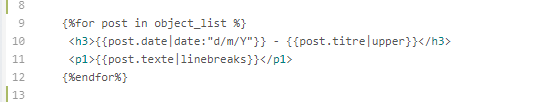
\includegraphics[scale = 1]{boucle_for.png}
\smallbreak
Boucle for
\end{center}
\bigbreak
Les balises ligne 10 servent à donner la date et le titre de l’article et la ligne 11 sert à donner le texte lié à l’article en question. Cette boucle permet d’afficher tous les articles à la suite. Ces articles se trouvent sur la page d’accueil du site.
\bigbreak
Pour l'instant l’aspect design de la page est encore rudimentaire mais est déjà un plus pour cette soutenance. J’ai créé un Favicon afin d’en avoir un personnalisé et ajouté quelques couleurs pour que le site ne soit pas non plus juste du texte mal organisé. J’ai aussi ajouté une police d’écriture libre de droit pour le titre de notre site qui est bien sûr : \textit{The Believer’s Quest}.
\bigbreak
\begin{center}

\includegraphics[scale = 1]{image_TBQ.png}
\smallbreak
Favicon du site Web
\end{center}
\bigbreak
Une page Instagram a aussi été instaurée le 25 février afin de mettre des photos de nos graphismes et autres contenus intéressants.
\newpage

\subsection{Mars}
\bigbreak
\bigbreak

Du 9 au 11 mars, j’ai commencé à réaliser l'interface utilisateur du jeu. J’ai donc dû commencer par prendre en main Unity et son module UI qui permet de faciliter la création de celle-ci. Nous avons décidé de créer une interface contenant :
\bigbreak
\begin{itemize}
\item Une jauge de vie qui serait en haut à gauche
\item Un texte en haut à gauche qui donnerait le nombre de 'Golds' et de 'Diamonds' (pour l'instant on affiche les diamants aussi en partie normale, plus tard cela sera que dans le hub)
\item Une image (pour l’instant juste un carré bleu) pour afficher le sprite de l’arme dans les mains, en bas à droite
\item Un texte donnant le nombre de balles restantes dans le chargeur et le nombre de balles totales
\end{itemize}
\bigbreak
A des fins purement expérimentales, pour tester si l’affichage des Gold fonctionne j’ai ajouté une barre qui permet de contrôler la valeur.
\bigbreak
\begin{center}
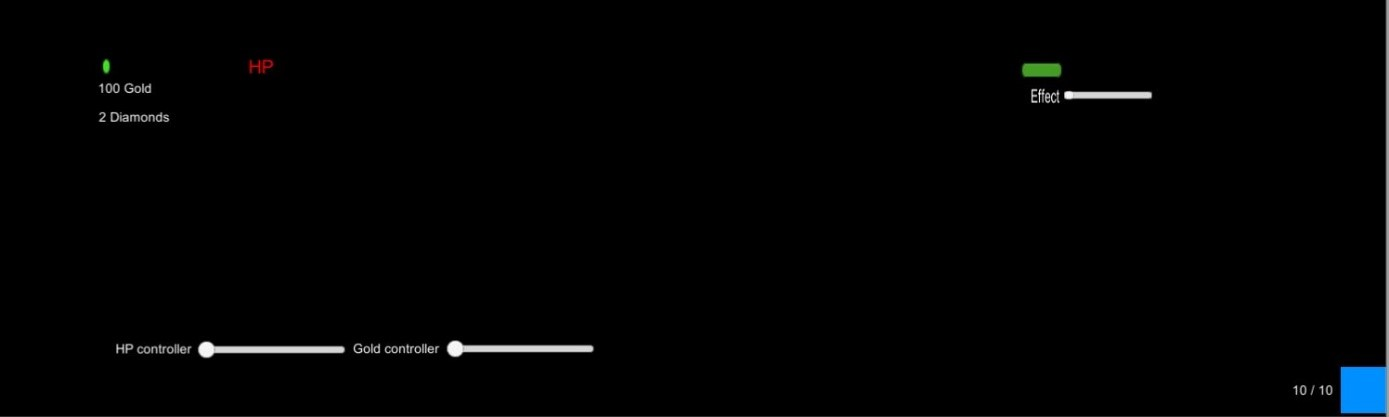
\includegraphics[scale = 0.32]{interface.jpg}
\smallbreak
Première interface
\end{center}
\bigbreak
Les 3 jauges blanches servent à contrôler les différentes valeurs pour les « HP », les « Gold » et la barre d’« Effect ». Ces jauges sont présentes afin de pouvoir tester si les valeurs s'affichent correctement sur l'écran, en effet elles augmentent les valeurs présentes dans le script.
\bigbreak 

\bigbreak
\bigbreak

Du 11 au 13 mars, j’ai consacré énormément de temps sur le site internet. J’ai donc passé beaucoup de mon temps à faire des recherches et des tests afin de réaliser la structure de notre site le mieux que possible et je suis satisfaite de celle-ci. J’ai commencé à travailler sur Unity seulement très récemment. J’ai eu énormément de mal à comprendre le fonctionnement de ce logiciel malgré des recherches et des vidéos regardées sur la prise en main de celui-ci. Pour l’interface utilisateur j’ai bien compris comment faire mais pour les attaques des ennemis et du joueur j’ai mis du temps à comprendre comment j’allais faire la chose. Le temps passé sur le site et ces difficultés m’ont contrainte à passer peu de temps sur les attaques.
\newpage

\section{Travail de Maxence Plantard}

\subsection{Janvier}
\bigbreak
\bigbreak
Avant même la date de rendue du cahier des charges, j’ai commencé à regarder les vidéos des tutoriels Unity pour pouvoir être efficace sur ce logiciel le moment venu.
\bigbreak
De plus je me suis en quête d’un logiciel pour faire de la musique facilement sur mon ordinateur. J’étais tout d’abord partager entre deux logiciels : Cubase et Bosca Ceoil. Néanmoins j’avais déjà utilisé un autre logiciel, Fruity Loop Studio 12. Malgré les difficultés d’adaptation au logiciel j’ai décidé de retourner sur Fruity Loop Studio.
\bigbreak
Dans les premières semaines du projet j’ai dû me documenter à propos de Unity et de FL Studio. En effet, j’ai mis quelques semaines à m’adapter aux modules de créations musicales les plus utilisés en matière de musique de jeux. N’ayant utilisé FL Studio que pour des musiques plus contemporaine comme de la pop ou autre musique électro, j’ai dû refaire tout mon stock d’instruments et d’effets sonores. Le plus facile pour faire une musique de jeu à mon avis est de faire un son basé sur une mélodie au clavier (piano ou synthétique) ou sur une mélodie orchestrale (cloches, violons ou autre instruments à vents).
\bigbreak
\bigbreak
\bigbreak
Le 22 Janvier, j’ai commencé la première composition seul. Je suis parti sur un ensemble de deux mélodies, l’une au violon et l’autre piano. En superposant les deux et en décalant les fréquences des différents sons, on obtient une mélodie douce et calme qui nous a tout de suite fait penser à une musique de menu. 
\newpage
Le 23 Janvier, lors de ce premier jour de travail en groupe sur le projet, j’ai commencé à travailler avec Nicolas. Nous avons utilisé pour cette fois uniquement le logiciel BoscaCeoil étant beaucoup plus intuitif et facile à prendre en main pour quelqu’un comme Nicolas qui n’a jamais fait de musiques. Au bout de deux heures de travail nous avons pu composer une première mélodie de base avec un piano aigue.
\bigbreak
\bigbreak
\begin{center}
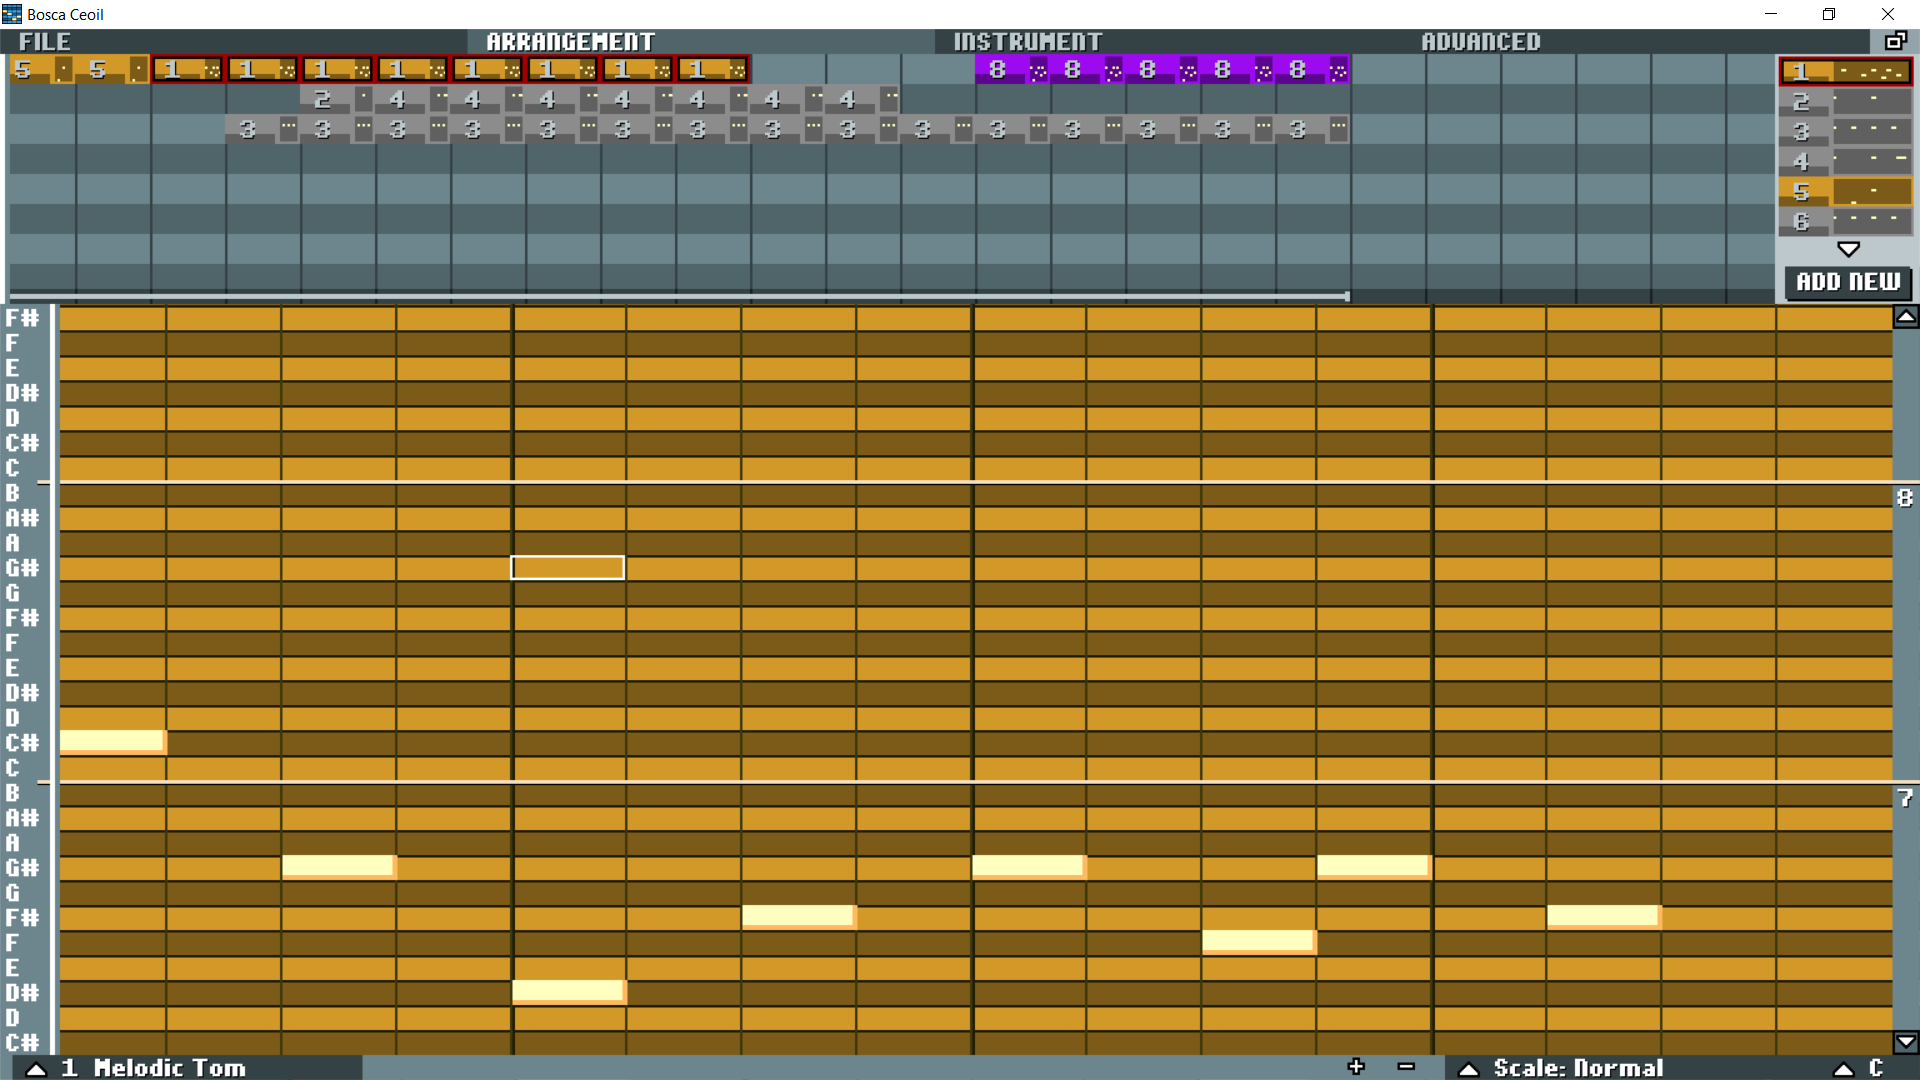
\includegraphics[scale = 0.18]{ceoil.png}
\bigbreak
Logiciel de musique Bosca Ceoil
\end{center}
\bigbreak
\bigbreak
Le 24 Janvier, j’ai retravaillé la mélodie du 23 pour y ajouter une ligne de percussions avec une caisse claire et une grosse caisse. J’ai ensuite ajouté un break ou j’ai enlevé le piano pour marquer un arrêt avant la suite du morceau. Après le break j’ai relancé la même mélodie composée le jour d’avant en montant chaque note d’une octave pour obtenir un son entrainant, joyeux et énergétique. 
\newpage

\subsection{Février}
\bigbreak
\bigbreak
Le 1er Février, je me suis mis à travailler sur un nouveau morceau, plus grave, plus sombre. Nos deux premières musiques étant plus réserver au menu et à la musique du hub ou du shop voir du premier niveau, ma volonté pour cette nouvelle composition était de créer un morceau plus proche d’un rogue like. Je rappelle que le joueur parcours des souterrains pour achever sa quête, une musique plus sombre et plus sérieux était donc plus adéquate. J’ai commencé par chercher un instrument convenable pour faire ce morceau. J’ai choisis un synthé grave accompagné de percussion à la fois commune comme un kick basique venant d’une simple grosse caisse ou encore un 808 Ch qui correspond à un charlestone. Néanmoins pour créer une atmosphère plus pesante j’ai choisis d’utiliser des WoodBlock et des œufs qui sonnent plus atypiques que d’autres instruments.
\bigbreak
Le 8 Février, après une semaine sans inspiration j’ai décidé de reprendre le morceau du 1 février. J’ai mixé le morceau pour que tous les instruments soient un peu en accord et que les fréquences ne soient pas trop mélangées.
\bigbreak
Les semaines suivantes j’ai réalisé de nombreuses maquettes. Néanmoins aucune ne semblait convenir aux besoins du groupe. De plus, je n’ai jamais essayé de faire de musiques de jeux avant ce projet donc je dois passer beaucoup de temps à écouter d’autres musiques de jeux et apprendre à les réaliser proprement.
\bigbreak
\begin{center}
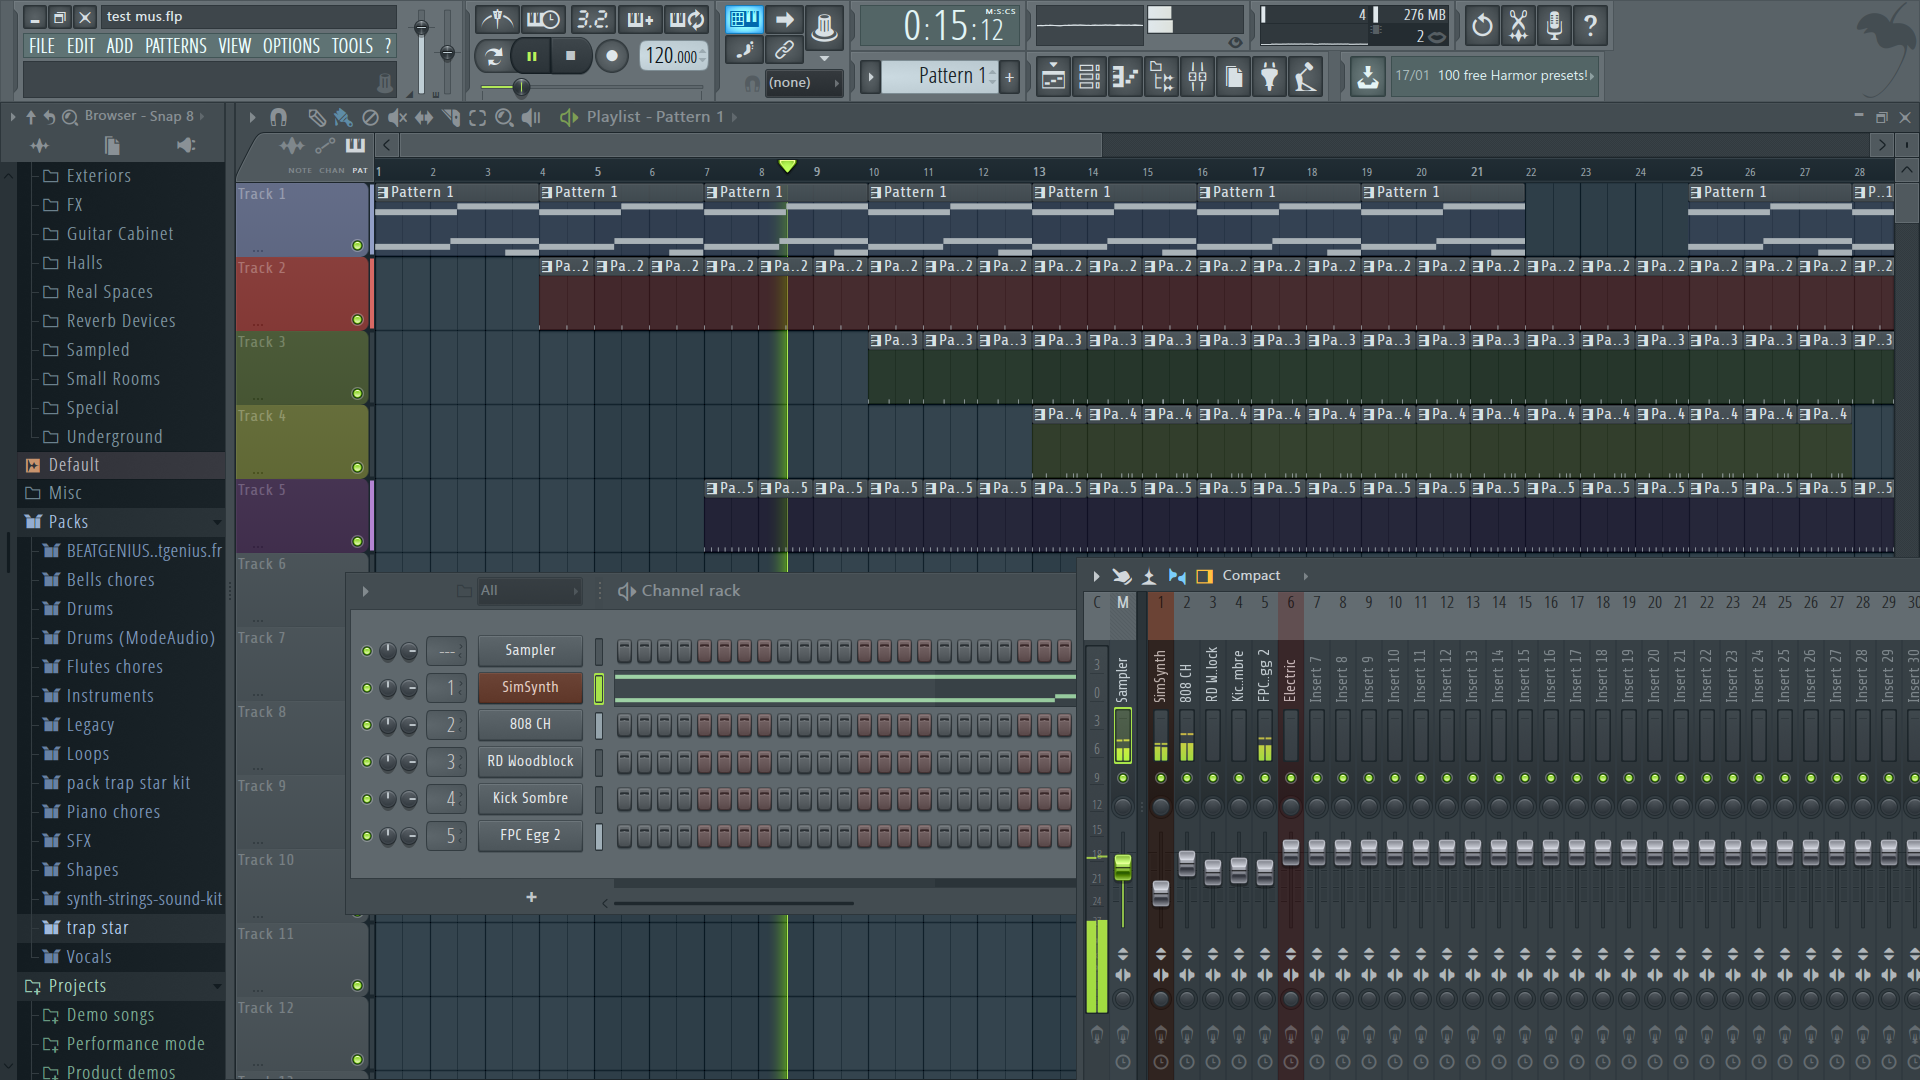
\includegraphics[scale = 0.18]{fruitloop.png}
\bigbreak
Logiciel de musique FLStudio
\end{center}
\bigbreak
N’ayant pas eu d’inspiration pendant trois semaines j’ai eu plus de temps à consacrer à la réalisation du projet. 
\newpage

Le 23 Février, Nicolas m’a montré ce qu’il avait fait pour les déplacements puis nous avons cherché à régler différents problèmes. Nous avons implémenté une solution pour gérer la vitesse du joueur.
\bigbreak
\bigbreak
Fin Février, j’ai commencé à me renseigner sur les déplacements des adversaires. Le pathfinding est en effet une partie compliquée du déplacement des ennemies vers notre joueur. J’ai ainsi fait des recherches sur le module Pathfinding et l’IA de Unity. Néanmoins, nous n’avons pas commencé directement le développement du déplacement des adversaires.
\bigbreak
\bigbreak
\bigbreak
\bigbreak

\subsection{Mars}
\bigbreak
\bigbreak
Du 10 au 13 mars, j’ai revu avec Nicolas tous les déplacements qu’il avait codés. De plus, nous avons cherché des idées pour le déplacement des adversaires. Dans un premier temps nous avons voulu déplacé l’ennemi sans nous préoccuper des collisions avec les murs. Nous nous basons sur les coordonnées du joueur puis utilisons une fonction pour envoyer l’ennemi vers le personnage. 
\bigbreak
Pour la détection du chemin à prendre avec les collisions nous envisageons d’utiliser le module PathFinding de Unity. Néanmoins nous n’avons pas encore commencé cette partie du code.
\bigbreak
Après près de deux mois sur le projet, je connais les difficultés pour réaliser différents morceaux pour un jeu vidéo. De plus, la musique n’est pas le seul besoin audio du jeu. En effet, je dois aussi réaliser tous les effets sonores comme ceux des armes ou des monstres ou encore les bruits de pas. Je pense que la documentation pour ce genre de bruitage sera plus fournie que celle pour la création des musiques car je n’ai pas encore trouvé la formule magique pour faire un morceau correspond parfaitement à un niveau ou à un ennemi. 
\bigbreak
Néanmoins je ne peux pas réduire mon expérience sur ces deux premiers mois à de longues séances de blancs sans inspiration. Composer des musiques reste un moyen ludique de participer au projet même s’il demande plus de temps que d’autres parties. Le problème majeur contrairement au code est de trouver ce que l’on doit faire alors que par exemple pour le pathfinding nous avons déjà nos idées.
\bigbreak
Je vais maintenant essayer de rendre un morceau par semaine pour combler tous les niveaux et tous les combats de boss. Il me faut aussi une musique de fin, pour le menu et pour le magasin. 
\bigbreak
De plus, je vais attaquer le développement du magasin et mettre au propre nos différentes idées pour le déplacement des entités adverses.
\newpage

\section{Travail de Nicolas Indjein}

\subsection{Janvier}
\bigbreak
\bigbreak

Même si le projet n’était à cette date pas encore accepté, j’avais la volonté de commencer à préparer le terrain. Dès le 19 janvier, j’ai donc commencé les classes Player, Ennemy et Weapons. Leur contenu était alors très basique. Le but était de commencer à structurer ce qu'il faudrait faire ensuite en créant des méthodes de bases qui seraient nécessaire dans le futur, mais qui ne nécessitaient pas de trop grandes réflexions (exemple : méthodes d’accès aux attributs des classes). C’est aussi à ce moment que j'ai commencé à regarder l’ensemble des vidéos de tutoriels sur le scripting en Unity.
\bigbreak

\bigbreak
\bigbreak

Le site avait commencé par être réalisé en tant que site statique. Cependant nous nous sommes ensuite tournés vers un site dynamique à la vue des avantages que cela procure. Le 21 janvier, j'ai donc commencé à créer le projet Django et à adapter les fichiers HTML pour commencer le transfert vers le mode dynamique. C'est aussi à partir de ce jour que les problèmes ont commencé.  Nous n'avions pas tous utilisés la même version d'Unity pour éditer le projet. Cela a évidemment entraîné des conflits de fusion des fichiers sur Git. Bien que Git soit bien fait et marque les endroits qui génèrent les conflits, je ne pouvais pas régler ces problèmes à la main car je ne comprenais pas ce qu'il y avait écrit dans les fichiers. J’ai donc pris la décision de supprimer le dépôt Git et d’en créer un nouveau.
\bigbreak


\bigbreak
\bigbreak
N’ayant jamais utilisé une tablette graphique et le logiciel Krita, c'est le 26 janvier qu'il m'a paru nécessaire de commencer à faire le logo du groupe et le fond d'écran du site assez promptement. Le logo du groupe a été réalisé rapidement, à l'opposé de la coupe qui, après plusieurs jours de travail, n'est alors toujours pas achevée. Par ailleurs je n’y ai pas touché depuis car après cette date j'ai préféré me concentrer sur le projet en lui-même. Cependant, à part quelques affinages potentiels à réaliser et peut-être quelques détails à rajouter, il ne reste que l'ombrage à réaliser. Ci-après la coupe dans son état actuel. 
\bigbreak
\begin{center}
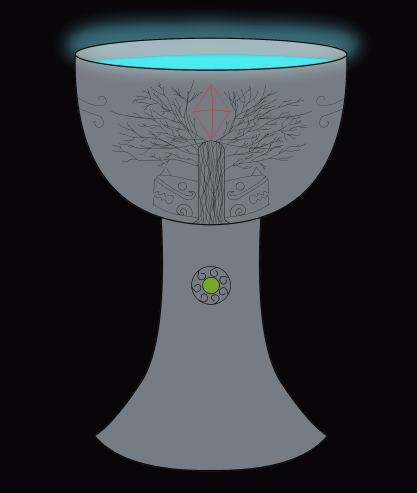
\includegraphics[scale = 0.3]{coupe.png}
\end{center}

\newpage

\subsection{Février}

\bigbreak
\bigbreak
C'est le 9 février que j’ai commencé à programmer la génération des salles. Vu que nous n'avions pas de sprites à ce moment, j'ai utilisé des carrés de couleurs. Le but était de générer des salles disposées les unes à côté des autres de manière aléatoire. Le taille du plateau qui les contenait, leur taille et leur nombre sont modifiables. Très vite il s'est avéré que cela allait être plus compliqué que prévu. En effet, coder sous Unity est beaucoup plus difficile que de coder de manière lambda. Il est nécessaire de se plier aux exigences d'Unity et notamment des contraintes imposées par l'héritage de la classe de base du logiciel, MonoBehaviour.
\bigbreak
Le 10 février, sachant qu'il fallait que tous les sprites possèdent la même taille et aussi pour faciliter mon travail, j'ai tout d’abord créé une feuille de sprites type qui est composée de cases roses. Puis j'ai créé une feuille de sprites qui me permettrait de réaliser les prototypes de mes sprites. J'ai ensuite commencé à imaginer et à donner forme à quelques sprites. Pour concevoir un sprite (sauf pour ceux des décors), je travaille toujours de la même façon. Tout d'abord je fais des esquisses de mes idées sur papier. Je choisis ensuite celles qui me plaît le plus. J’envoie ensuite une photo aux autres membres de mon groupe pour avoir leur avis. S'il est favorable, je commence à faire le sprite. Lorsque j’arrive à un résultat acceptable, j’envoie ce que cela donne à mes camarades pour avoir à nouveau leur avis. Cela me permet de faire différentes retouches pour finalement arriver à un résultat qui convient à tous.
\bigbreak

\bigbreak
\bigbreak

Le 27 février, j'ai travaillé sur la résolution des problèmes de scripts pour la génération d’un étage. Les salles sont désormais collées après beaucoup de problèmes rencontrés. Bugs de porte à corriger et murs à coller.
\bigbreak
Le 28 février, au bout de quelques tests il s'est avéré qu'il y avait un bug au niveau de la génération des salles. Il arrivait qu'elles ne soient pas du tout collées. Cela était dû à la manière dont fonctionnait l’algorithme à l’époque. En effet ce-dernier utilisait un tableau dans lequel des booléens représentaient si oui ou non une salle existait à tel emplacement. Les salles étants créées une à une, le problème venait de la détection de si une salle était déjà présente à un emplacement testé pour la nouvelle salle. N’ayant pas de debugger sous Unity et vu qu'il paraît compliqué de lancer un script pour Unity en dehors du logiciel pour profiter du debugger de VisualStudio, j’ai créé une classe Utility. Cette classe a pour but de regrouper des méthodes utilitaires pour nous aider à développer. A la vue de mon problème, j'ai créé une méthode permettant d’afficher un tableau dans la console d'Unity pour pouvoir régler les bugs apparaissant lorsque le jeu est lancé. 
\bigbreak
Comme cela est visible au-dessus, les « portes » n’apparaissaient pas des deux côtés du mur. Une simple ligne de code supplémentaire aura réglé ce problème.
\newpage

\subsection{Mars}
\bigbreak
\bigbreak
Le 2 mars, j'ai pu corriger le bug de boucle infinie (génération de salle). Sprites murs terminés.
\bigbreak
Une hypothèse de bug probable avait été réalisée à la vue du code alors réalisé. Cette hypothèse s’est vue avérée au bout de quelques tests. Si tous les emplacements autour d'une salle étaient remplis, le code rentrait dans une boucle infinie. Ce bug est à ce jour l’un des plus long à corriger que j’ai rencontré dans ce projet. J'ai aussi fini les sprites de murs pour qu’on puisse tester la génération avec eux, et donc voir s'ils nécessitaient des modifications ou s'ils étaient déjà bons pour le jeu. Evidemment il s'est avéré qu'il fallait apporter des retouches, ce qui a été fait immédiatement. Cependant, en jeu les images étaient floues. Ce n'est que quelques jours plus tard que j'ai trouvé comment corriger cela.

\bigbreak
\bigbreak
Le 7 mars, j'ai créé un nouvel algorithme de génération de salle : plus efficace et portes positionnées en fonction des enfants et des parents de chaque salle. Modification supplémentaire : les salles sont désormais des objets fils de l’objet Board. Ajouts d’une classe utilitaire.
\bigbreak
Je trouvais que mon algorithme de génération de salle n'était pas « propre » et mal optimisé. Une autre manière de faire cette génération, plus propre, plus optimisée et plus compréhensible, a germé dans mon esprit et je l'ai donc implémentée. Étonnamment cela a fonctionné du premier coup. J'ai donc pu supprimer l’ancienne version. Cela a aussi été l'occasion de rajouter des méthodes dans la classe Utility pour afficher le temps d’exécution d’une partie du code dans la console d'Unity.
\bigbreak
C'est le 9 mars que j'ai commencé à faire des recherches pour la réalisation de l'interface (UI) même si ce n’est pas dans le travail qui m'est attribué car Sarah et Maxence était concentrés sur d'autres parties du projet et je voulais commencer à créer une interface de développement permettant de modifier les différentes variables en cours de jeu pour nous aider dans nos tests. De plus, le développement de l'UI me concerne aussi par rapport à l'aspect graphique de l’interface. J'ai donc commencé l'UI du joueur, en ajoutant la jauge d'effet, et l'UI de développement en ajoutant un slider pour modifier l'attribut correspondant au pourcentage d'effet.
\newpage

Le 11 mars, j'ai fini les sprites du joueur, et je les ai découpés pour l'animation.
 \bigbreak
\begin{center}
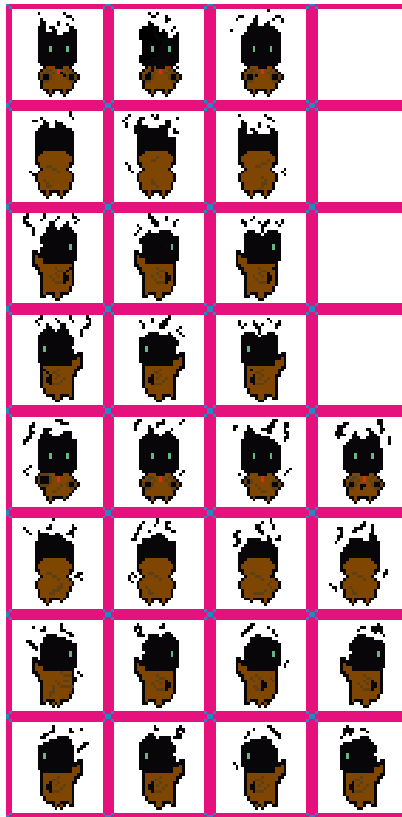
\includegraphics[scale = 0.25]{spritePerso.png}
\bigbreak
Sprites actuelles du joueur
\end{center}
\bigbreak
Cette journée a été difficile à cause des différents défis rencontrés. Tout d'abord le temps. J'étais en retard au niveau des sprites et j’ai donc été contraint de réaliser tous les sprites d'animations en un après-midi. A cela c’est ajouté un problème imprévu. Lors des transferts par Git, les modifications apportées aux objets dans la hiérarchie (c'est-à-dire les objets ajoutés à la scène dans Unity) n'étaient pas envoyées sur le dépôt. J'ai donc changé le .gitignore pour que ces modifications soient transférées. Cependant Unity modifie en permanence certains fichiers et les recrée s'ils ont disparu. Mais si le fichier existe et qu'il a été modifié depuis Unity mais sur un autre PC cela entraîne des conflits. Ces fichiers en font partie. En plus d’avoir des conflits de fusion sur Git il y avait donc en plus des problèmes avec Unity, ce qui avait totalement cassé le projet. Même la fusion de la branche de backup avec la branche de travail ne fonctionnait pas. Après 2h de tentatives pour réparer tous ces problèmes, j'ai été contraint d'abandonner et de tous supprimer dans le dépôt, puis de renvoyer une ancienne version du projet. Malgré ce gros problème m'ayant fait perdre beaucoup de temps, j'ai réussi à faire tout ce qu'il fallait.
\bigbreak
Le 12 mars, un autre problème est survenu. Nicolas m’a prévenu que l’objet du joueur dans Unity était repésenté comme un fichier invalide. En me penchant sur le problème j’ai découvert que le fichier avit été corrompu à cause d’une fusion raté. Ne sachant ni d’où venait le problème, ni comment le régler rapidement, j’ai supprimé et recréé l’objet en espérant que ce bug ne surviendrait plus. Heureusement Nicolas m’a informé que pour l’instant il n’y avait pas l’air d’y avoir de problèmes.
\newpage


\section{Travail de Nicolas Lorrain}

\subsection{Janvier}
\bigbreak
\bigbreak
Le mois de Janvier s’est principalement composé d’une étude approfondie d’Unity et de ses caractéristiques. Unity, malgré l’utilisation de C\#, est très déroutant parce qu’il relie les scripts et l’interface du logiciel. Même si une fois la logique apprise, tout cela semble évident, c’est assez compliqué de comprendre les tenants et aboutissants. 
\bigbreak
J’ai donc, pour apprendre Unity, regardé différents tutoriels, certains officiels, d’autres officieux. Dans les tutos officiels trouvables sur le site Unity, on retrouve notamment :
\bigbreak
\begin{itemize}
\item Le tutoriel officiel appelé « Scripting », qui permet de comprendre de façon global le logiciel.
\item Le tutoriel 2D roguelike, qui se rapproche plus de notre jeu (mais qui ne s’avèrera pas si semblable au fil du temps).
\end{itemize}
Dans les tutoriels officieux, on retrouve :
\bigbreak
\begin{itemize}
\item Une liste de vidéos appelée « Apprendre le C\# (Unity 3D) » sur YouTube, qui rappelle les bases du C\# mais agrémenté de notions liées à Unity.
\end{itemize}
\bigbreak
Ces vidéos m’ont été très utiles et il faut l’avouer m’ont permis de retarder le moment du codage. Car c’est vers cette période où on s’intéresse à Unity, on apprend les ficelles du logiciel, et on se rend compte que ce ne sera pas si facile. Je me suis un peu demandé si notre cahier des charges n’était pas trop ambitieux. 
\bigbreak
Néanmoins, nous n’avons pas décidé de revoir notre planning à la baisse et avons décidé de le suivre. Nous savions que le résultat au moment de la première soutenance serait de toutes façons différent du résultat escompté.
\bigbreak

\bigbreak
\bigbreak

 Le 16 janvier, en parallèle de la documentation Unity, nous avons évidemment travaillé sur le cahier des charges. J’étais personnellement en charge de la mise en page, et donc de l’utilisation de Latex. J’ai utilisé le logiciel MikTek.
\bigbreak
Malgré mes réticences initiales, je suis rentré dans Latex assez rapidement et j’ai assez vite compris. Il m’aura fallu quelques recherches Internet pour trouver les différentes façons de mettre en page.
\bigbreak
Le 17 janvier, j’ai fini la mise en page du cahier des charges. Le PDF de la première version est prêt.
\bigbreak
Le 18 janvier, j’ai fait certaines modifications de dernière minute. Par exemple, j’ai rajouté le fait que le joueur pourra donner un nom à son personnage. Cela clos le travail sur cette version du cahier des charges, puisqu’il est remis en fin d’après-midi.
\bigbreak

\bigbreak
\bigbreak 
Le 23 janvier, j’ai travaillé avec Maxence sur la musique. Nous avons notamment travaillé sur une musique que nous considérons convenable pour plus tard. Nous nous sommes aussi dit que la musique du boss final pourrait reprendre la musique du hubmais avec un tempo et une ambiance différente.
\bigbreak
Le problème ici fut que je n’avais aucune connaissance en logiciel de musique et en musique de façon plus générale, donc je servais surtout de seconde oreille à Maxence. J’étais là pour lui donner quelques idées mais c’est lui qui faisait la majorité du travail. 
\bigbreak

\bigbreak
\bigbreak
Le 29 janvier, j’ai enfin commencé à coder : je me suis penché sur la génération de salle. Tout en me basant sur les fondations de code créées par Nicolas Indjein, j’ai débuté par une génération basique, c’est-à-dire un sol et des murs en fonctions d’une longueur et d’une largeur prédéfinies. 
\bigbreak
Pour cela, il aura fallu une double boucle toute simple qui fait apparaitre un GameObject Mur quand on se trouve sur les côtés et un GameObject Sol le reste du temps. 
\bigbreak
\begin{center}
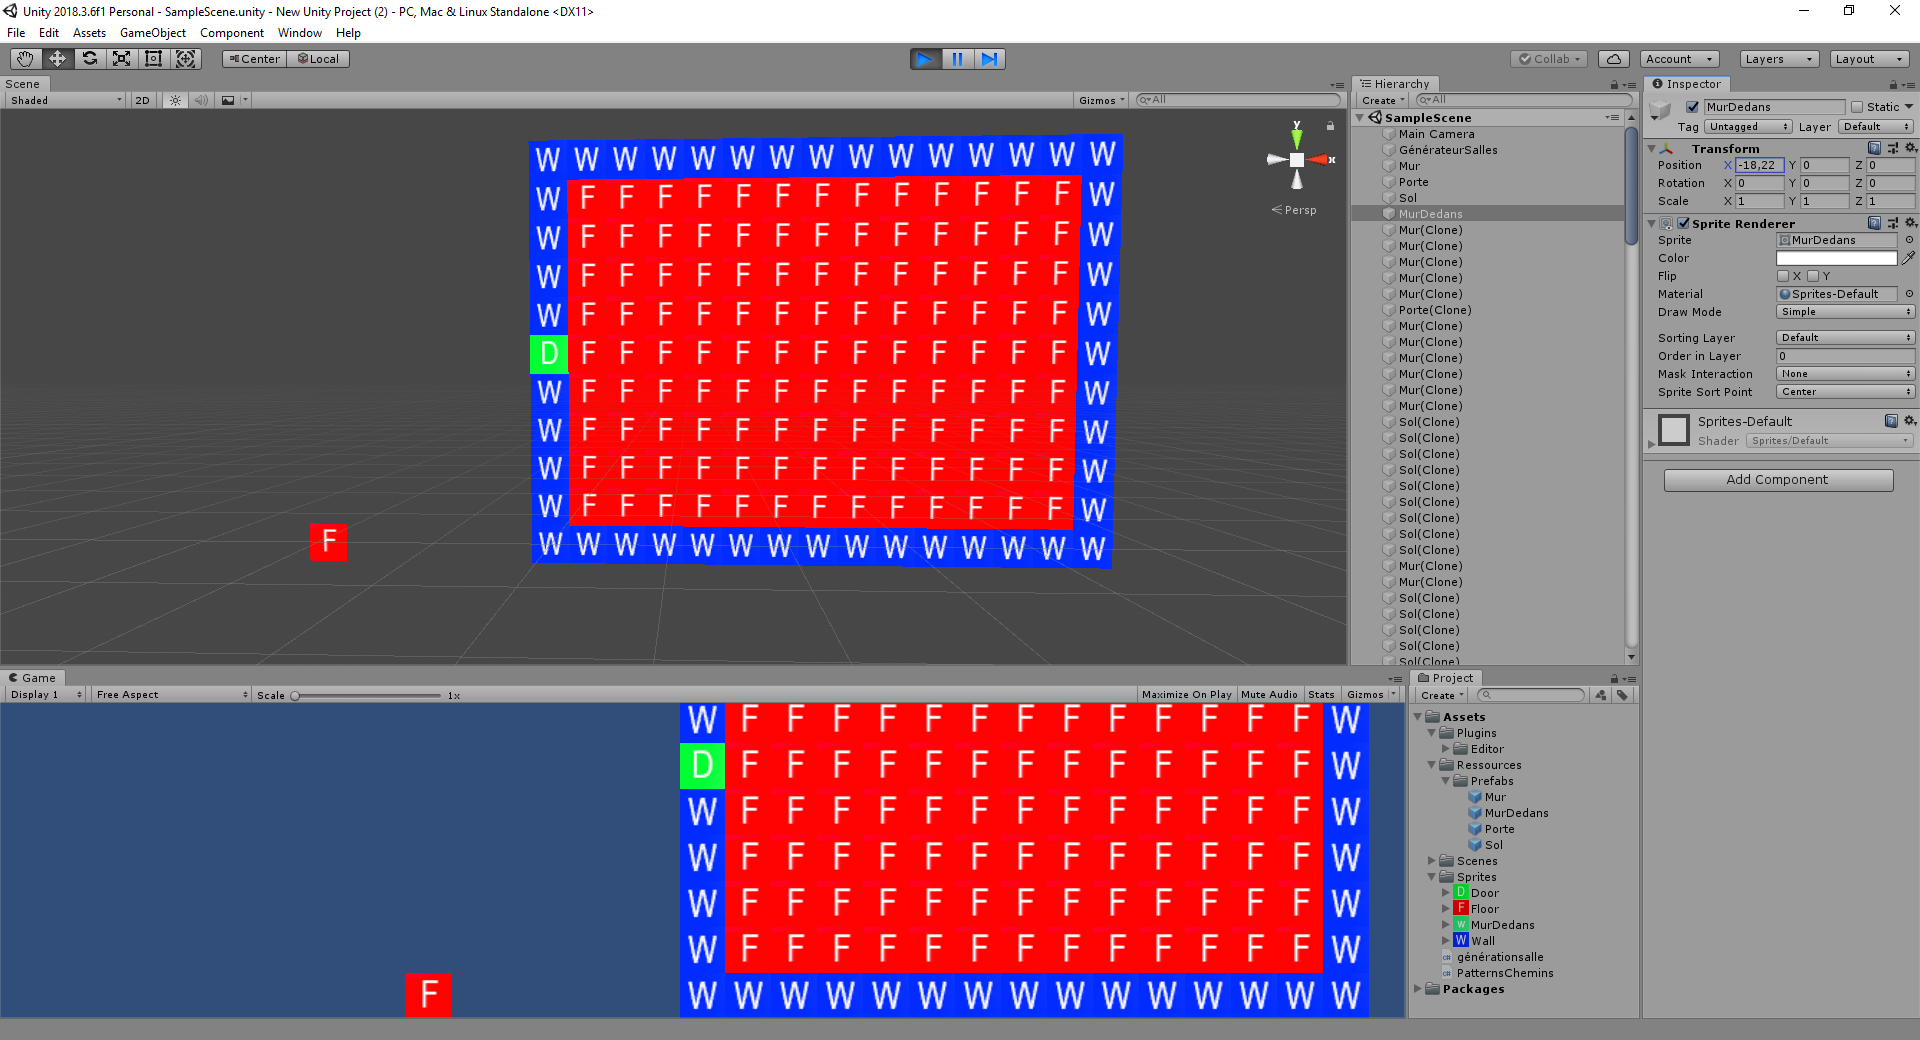
\includegraphics[scale = 0.23]{generation.PNG}
\bigbreak
Génération d'une salle sans sprites sous Unity
\end{center}
\bigbreak
\bigbreak
Cependant, malgré la simplicité du code, j’ai eu quelques soucis d’intuition, notamment au niveau des liens entre Unity et le script. C’était ma première expérience « sur le terrain » et même avec les connaissances acquises en regardant des vidéos je n’étais pas entrainé.
\bigbreak
J’ai réussi au bout de quelques heures à atteindre le résultat de la capture d'écran, à l’aide de sprites d’une seule couleur.
\bigbreak
Le 30 janvier, j’ai continué mon étude d’Unity une bonne fois pour toutes être à l’aise avec le logiciel.  
\bigbreak
J’ai ensuite continué mon travail sur la génération de salles, et plus particulièrement sur l’apparition d’une porte. J’ai réussi cela sans problème, en considérant que la porte se situera au milieu d’un côté. 
\bigbreak
Tout le travail effectué jusqu’à présent sur la génération de salles fut ensuite utilisé et modifié par Nicolas Indjein pour qu’il crée finalement la génération de salles à sa manière.
\bigbreak

\subsection{Février}
\bigbreak
\bigbreak
C’est le 1 février qu’on nous a fait un compte-rendu du cahier des charges, pour que l’on puisse le modifier en fonction des critiques faites. Le 3 février, j’ai ainsi rajouté un paragraphe dans la partie « Etat de l’art » et j’ai mis le nom du groupe en évidence sur la page de garde.
\bigbreak

\bigbreak
\bigbreak

Le 17 février, j’ai travaillé sur un nouveau sujet : les déplacements du personnage. J’ai basé mon travail dans la classe Player.
\bigbreak
J’ai dans un premier temps voulu utiliser le principe des rigidbody. Je pensais qu’il fallait utiliser les rigidbody du personnage et le faire bouger à l’aide d’une force mais cela donnait un déplacement bizarre, comme si le personnage glissait. J’étais décontenancé au début, puis j’appris l’existence des colliders.
\bigbreak
Cependant, l’un de nos niveaux prévus est un niveau de glace, où le personnage devrait glisser sur certains blocs. J’ai donc gardé ce code de côté pour plus tard
\bigbreak
Finalement, j’ai utilisé différentes conditions qui vérifient à l’aide de Input.GetKey si les touches de déplacement (de base les flèches directionnelles) sont appuyés. Au départ, j’avais mis des « else if » entre chaque condition, mais cela posait problème car seule une direction en même temps pouvait être pris en compte. Les diagonales ne fonctionnaient. J’ai ensuite compris le problème et j’ai réglé cela.
\bigbreak
J’ai finalement réussi à mettre en place les déplacements, et c’est très satisfaisant d’avoir un code qui fonctionne. J’ai bien dû passer 30min à juste se faire déplacer ce cube qui deviendra bientôt notre personnage.
\bigbreak

\bigbreak
\bigbreak
Le 23 février, j’ai retravaillé sur les déplacements car il y a eu un problème avec git. J’ai donc réglé ces quelques problèmes de conflit et j’ai aussi calibré la vitesse du joueur pour qu’elle semble plus ou moins réaliste.
\bigbreak

\bigbreak
\bigbreak
Le 28 février, les déplacements étant donc bien finis, je me suis penché sur les collisions entre le joueur et les murs. J’ai travaillé dans la classe MovingObject.
\bigbreak
Je me suis documenté sur les colliders à l’aide des vidéos citées plus hauts. Je me suis dit qu’évidemment il fallait utiliser cette fonctionnalité d’Unity pour coder les collisions. Au début, je pensais qu’il fallait tout simplement donner aux objets concernés le composant « Box Collider » mais je me suis vite rendu compte que c’était plus compliqué que ça.
\bigbreak
Ainsi s’est déroulé une soirée pleine de questionnements et de rage face à un code qui ne fonctionne pas. Après de nombreux essais, j’ai plutôt utilisé les composants « Box Collider 2D » plus adaptés à notre jeu. 
\bigbreak
\bigbreak

\subsection{Mars}
\bigbreak
Le 1er mars, j’ai de plus opté pour l’utilisation d’un RaycastHit 2D (une ligne invisible qui peut détecter des boites de collision), qui part du centre du cube et se dirige vers une direction en fonction de la touche appuyé par le joueur. Si jamais ce raycast touche le collider d’un bloc, il change un booléen en faux, ce qui bloque le déplacement dans la fonction de déplacement de la classe Player. Pour cela, il a fallu que je fasse de Player une sous-classe de MovingObject (ce qui est logique après réflexion), pour pouvoir appeler la fonction de collision directement dans la classe Player.
\bigbreak
Cependant, j’ai fait face à un autre problème : les raycasts traversent les murs sans détecter de collision. Mais je reste persuadé que les raycasts sont la meilleure solution pour les collisions. Je me rends compte avec dépit que le problème était tout simplement que les blocs n’avaient pas sauvegardé leur composant « Box Collider 2D », car je les avais rajoutés à partir de la hiérarchie dans Unity et pas à partir des préfabs. Ce problème d’Unity m’aura causé du fil à retordre à plusieurs reprises, sans vraiment m’en rendre compte (en liant certains scripts à certains GameObjects par exemple).
\bigbreak
Le 10 mars, le raycast au milieu du personnage était opérationnel, mais je me suis rendu compte qu’au niveau du coin le cube qui nous servait de personnage rentrait quand même dans les murs. La solution était donc d’utiliser quatre raycasts partant des coins du cube : en détectant les collisions à l’aide des quatre, il était donc impossible que le cube traverse des blocs.
Quatre raycasts sont suffisants car on utilise des blocs dans notre jeu. De plus, nous n’avons pas besoin d’une précision extrême.
\bigbreak

Le 11 mars, le sprite du personnage ayant été implémenté dans le projet, j’ai dû calibrer les raycasts pour que la hitbox ait du sens par rapport au sprite plus « en longueur » du personnage.
\newpage

\section{Avances et retards du projet}
\bigbreak
\bigbreak
\bigbreak
\begin{itemize}
\item Site Internet : En ce qui concerne le site, nous sommes un peu en avance car du code CSS a été ajouter alors que l’objectif fixé était d’avoir une bonne structure de site et ensuite ajouter tout le web design. 
\bigbreak
\bigbreak
\item Communication : Les 10\% de communication ont été respectés. Le but était de créé les différentes pages et comptes du projet afin de permettre une base de notre communication. 
\bigbreak
\bigbreak
\item Interface : Cette partie est dans les temps car pour cette soutenance le but était d’avoir la structure de l’interface et de commencer à afficher les informations fondamentales à l’utilisateur. Ici toutes les informations ont été disposées comme elles se doivent aux endroits décidés. Les 20\% d’avancement annoncés sont donc bien respectés. 
\bigbreak
\bigbreak
\item Attaques : Pour les attaques du joueur et des ennemis nous sommes en retard, en effet pour l’instant les fonctions dans le script du joueur et de l’ennemi ne font que donner des dégâts et reste donc pour l’instant que très basique.
\end{itemize}
\newpage

\section{Ce qu'il faut faire pour la prochaine fois}
\bigbreak
\bigbreak
\begin{tabular}{|*{5}{c|}}
	\hline
	Tâches$\backslash$ Membre & Nicolas I & Sarah & Nicolas L & Maxence \\
	\hline	
	Sprites du 1er étage & X & & &  \\
	\hline
	Animations du 1er étage & X & & & \\
	\hline
	Patterns des salles & & & X & \\
	\hline
	Hitbox & & & X & X \\
	\hline
	Menu (options et principal) & & X & & \\
	\hline
	Attaques des ennemis du niveau 1 & X & X & & \\
	\hline
	Armes & X & X & & \\
	\hline
	Magasins & & & & X \\
	\hline
	Musiques du menu et du niveau 1 & & & & X\\
	\hline
	Sons du niveau 1 et des ennemis & & & & X \\
	\hline
	Transitions entre les niveaux & X & & X & \\
	\hline
	Hub & X & & X & \\
	\hline
\end{tabular}
\bigbreak
\bigbreak
\bigbreak
\bigbreak

\section{Conclusion}
\bigbreak
\bigbreak
Dans un premier temps, nous avons pris notre temps car nous ne pensions pas que coder sous Unity serait si différent. Mais après avoir eu autant d'erreurs sous Unity et après de très nombreuses recherches sur Internet, nous avons pris conscience de la difficulté de la chose. Nous nous rendons bien compte désormais du travail que nous aurons à fournir si nous voulons avoir un jeu complet. Voici un aperçu du jeu tel qu'il est à présent :
\bigbreak
\begin{center}
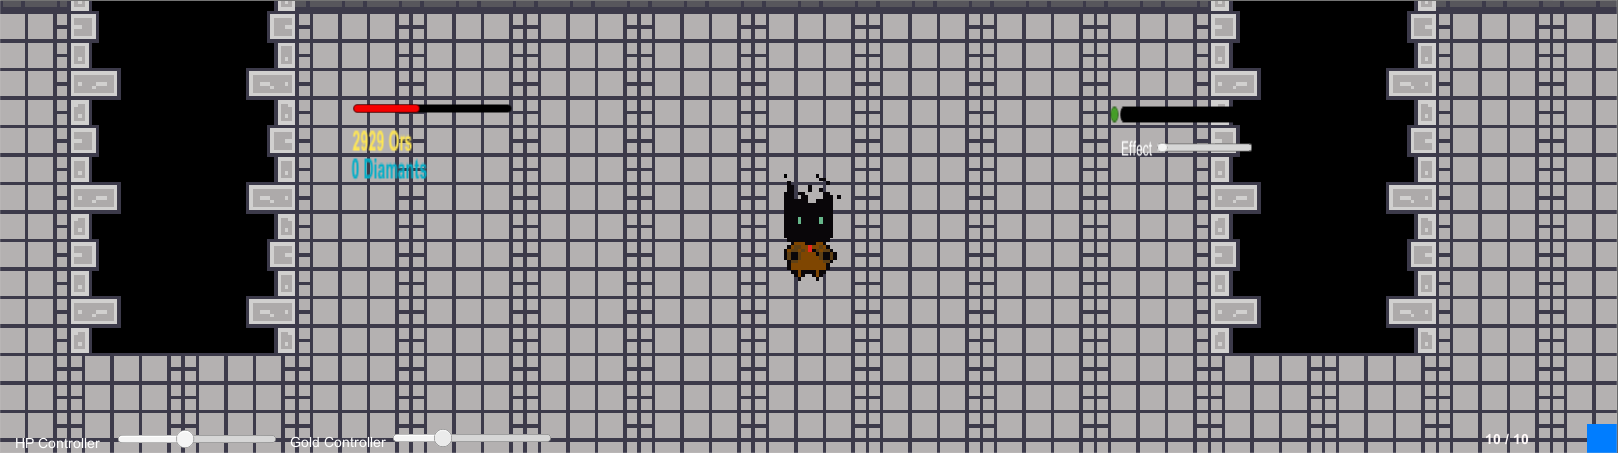
\includegraphics[scale = 0.35]{affichagejeu.PNG}
\end{center}
\end{spacing}
\newpage
\section{Annexe}
\bigbreak
\bigbreak
\begin{center}
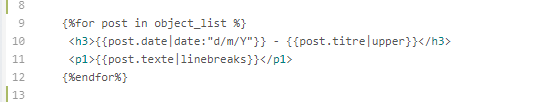
\includegraphics[scale = 1]{boucle_for.png}
\smallbreak
Figure 1 : Boucle for
\bigbreak
\bigbreak

\includegraphics[scale = 1]{image_TBQ.png}
\smallbreak
Figure 2 : Favicon du site Web
\bigbreak
\bigbreak
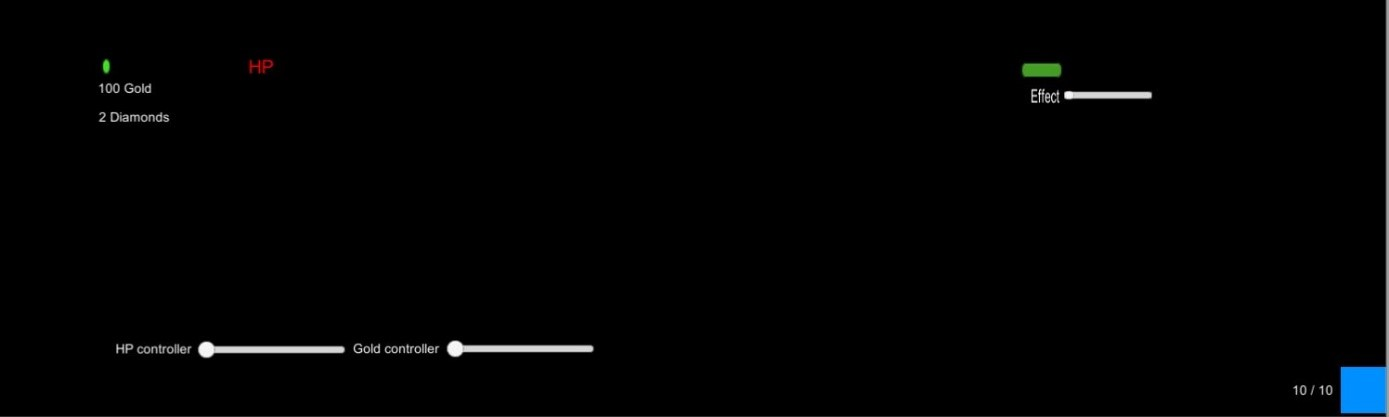
\includegraphics[scale = 0.32]{interface.jpg}
\smallbreak
Figure 3 : Première interface
\bigbreak
\bigbreak
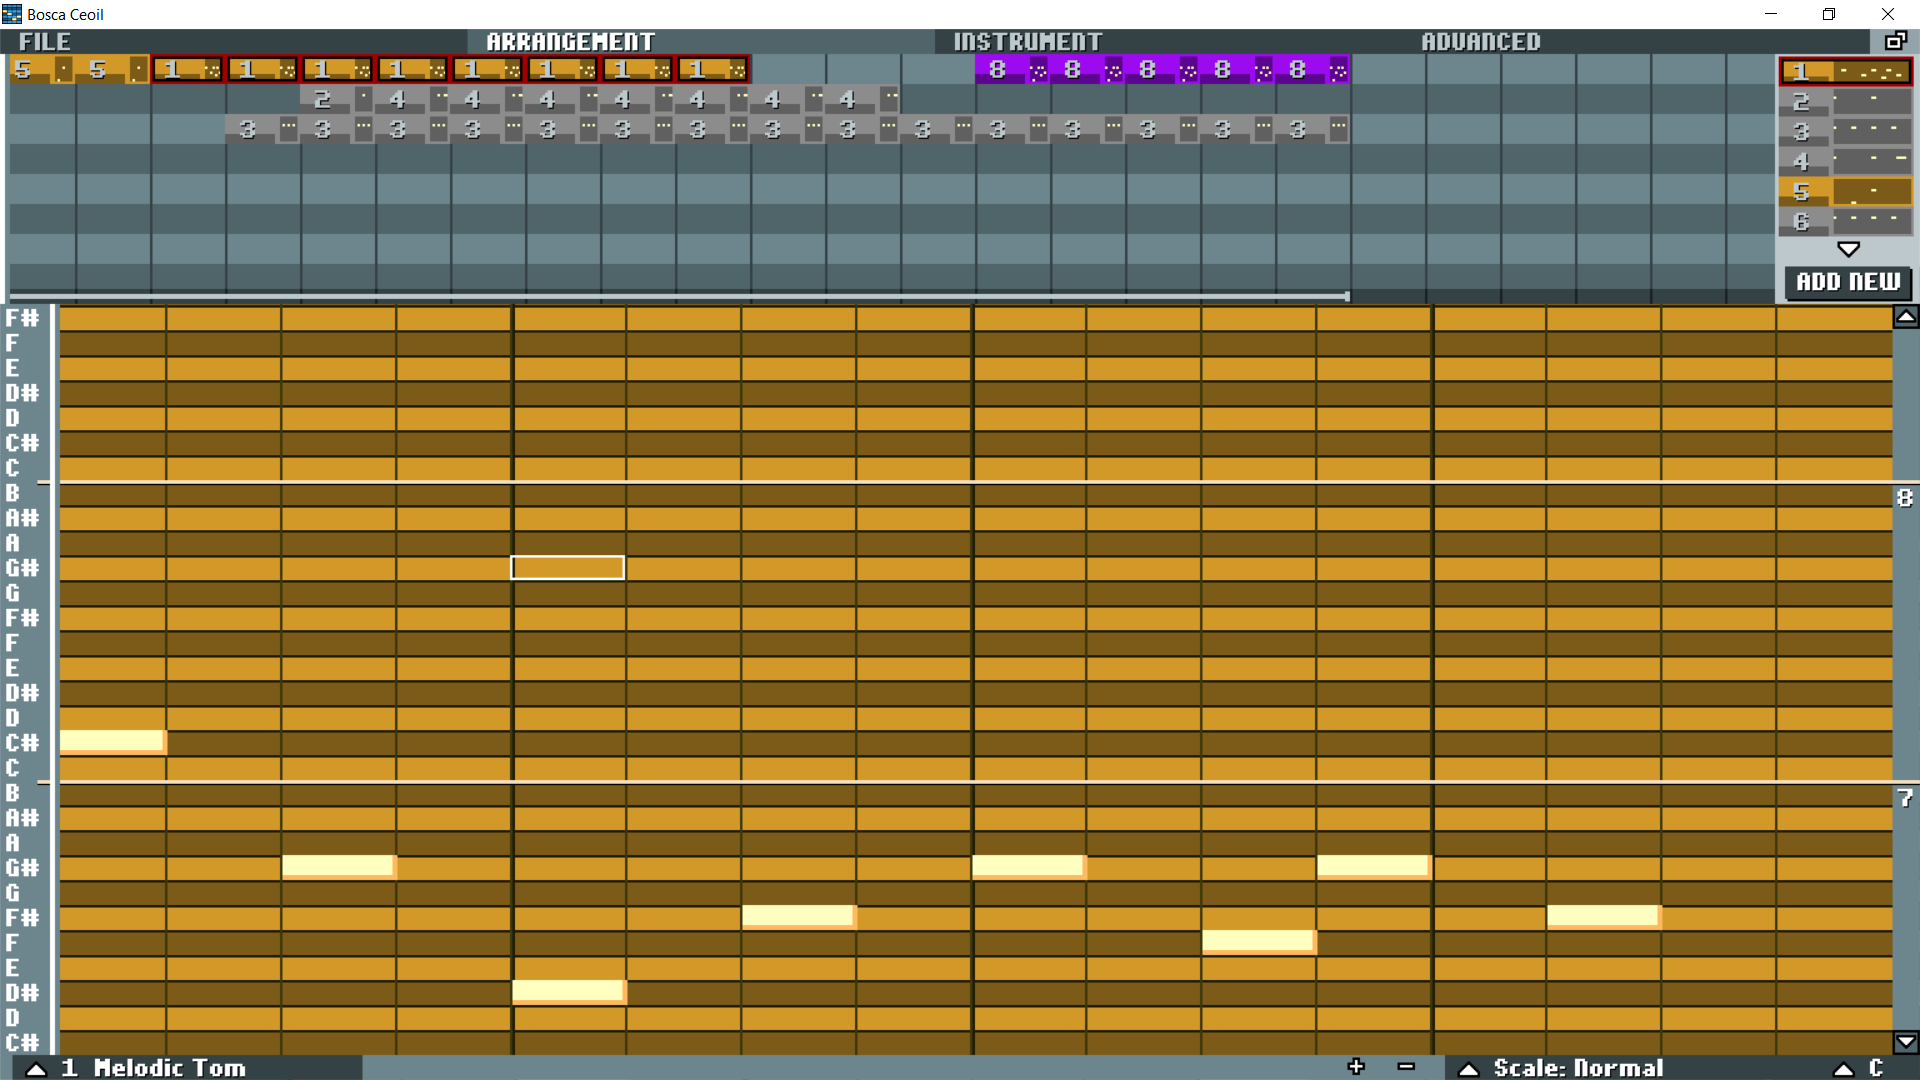
\includegraphics[scale = 0.18]{ceoil.png}
\smallbreak
Figure 4 : Logiciel de musique Bosca Ceoil
\bigbreak
\bigbreak
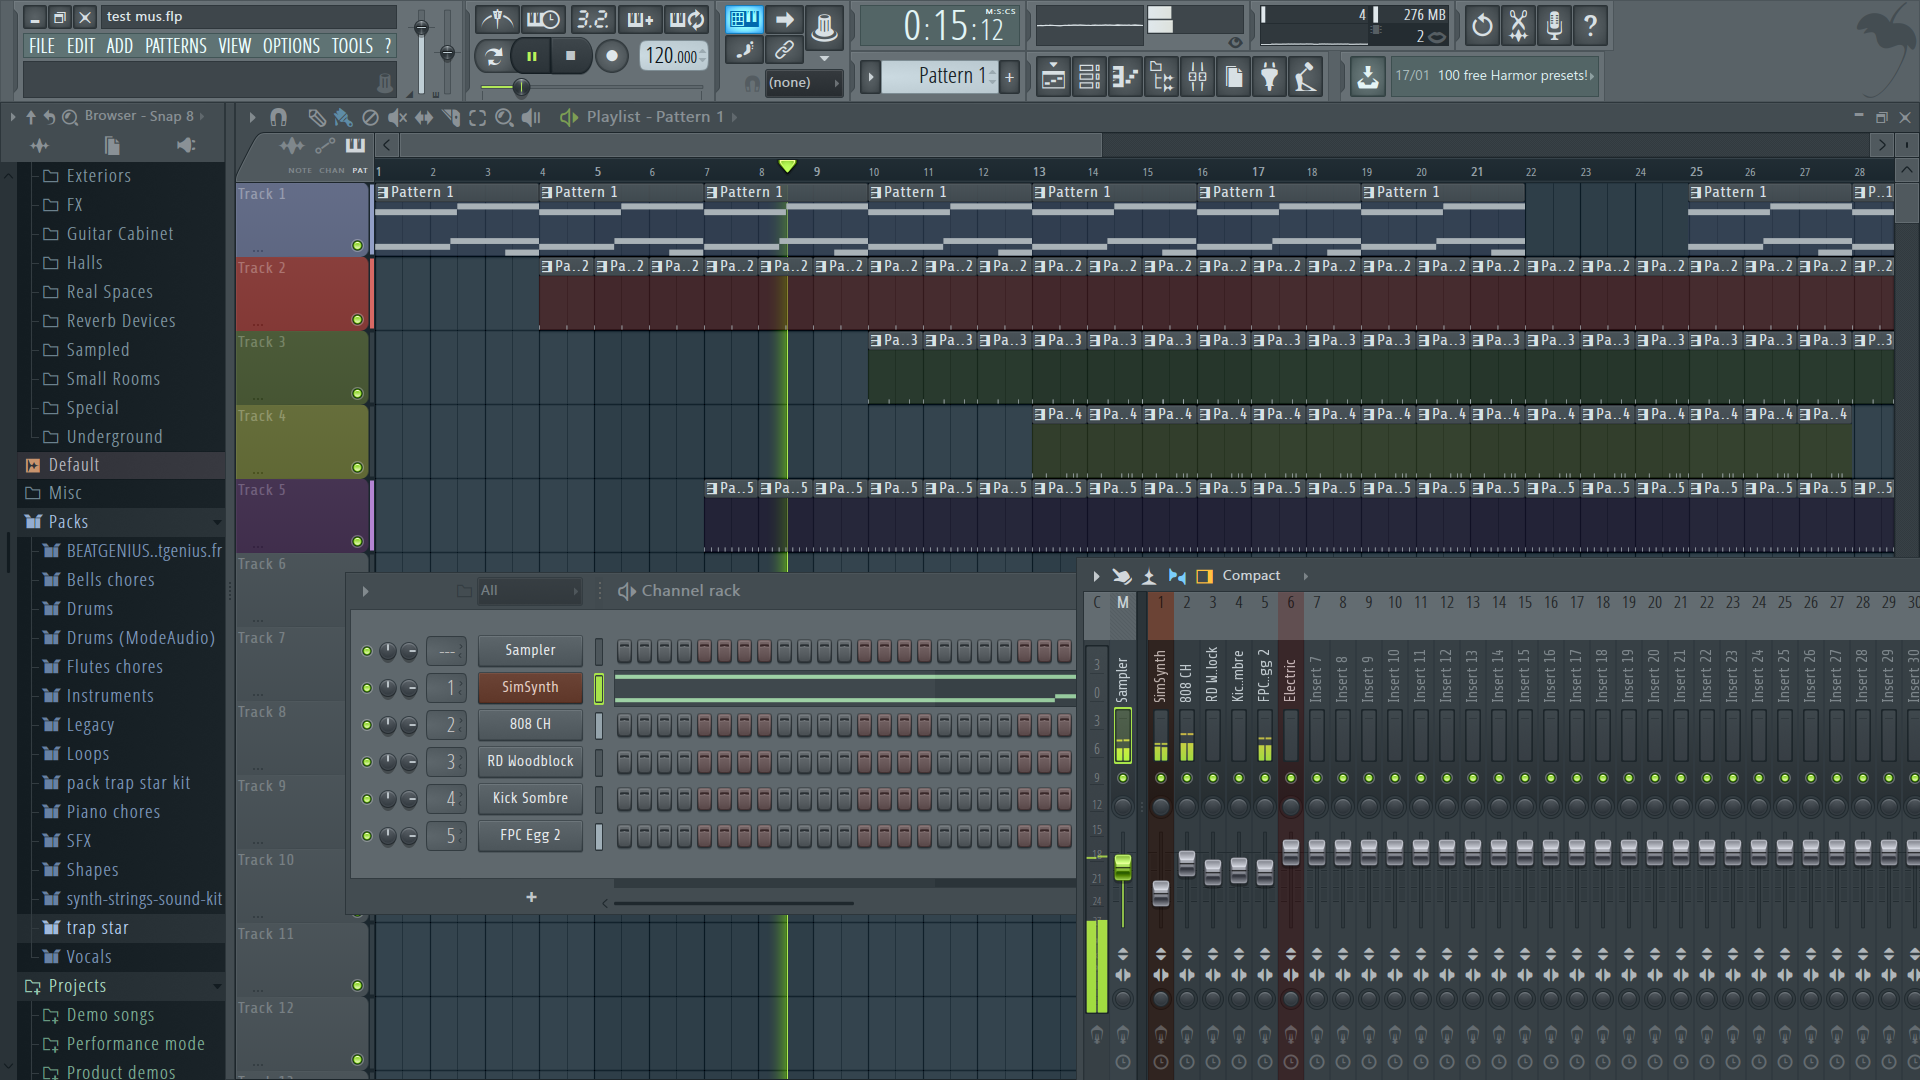
\includegraphics[scale = 0.18]{fruitloop.png}
\smallbreak
Figure 5 : Logiciel de musique FLStudio
\bigbreak
\bigbreak
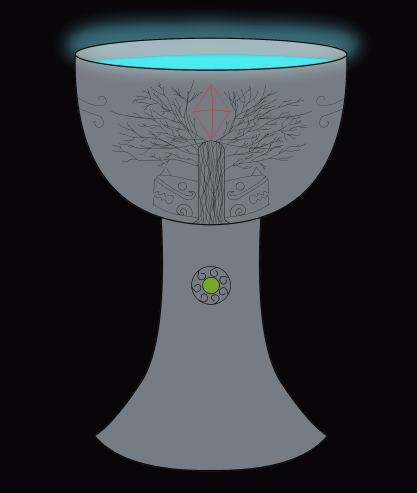
\includegraphics[scale = 0.3]{coupe.png}
\smallbreak
Figure 6 : Logo du groupe dans son état actuel
\bigbreak
\bigbreak
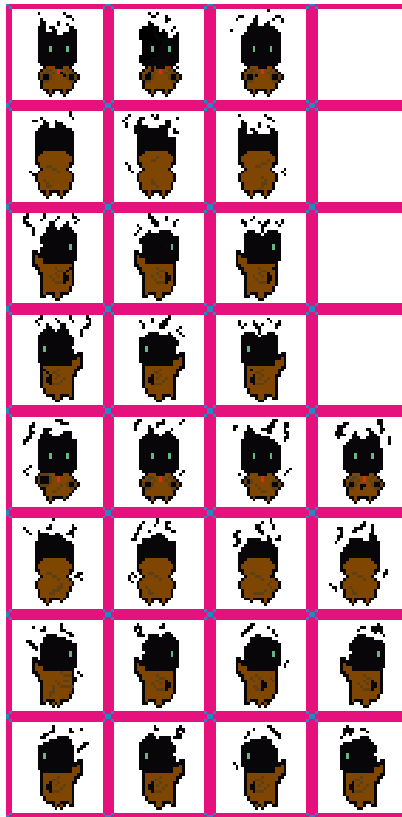
\includegraphics[scale = 0.25]{spritePerso.png}
\smallbreak
Figure 7 : Sprites actuelles du joueur
\bigbreak
\bigbreak
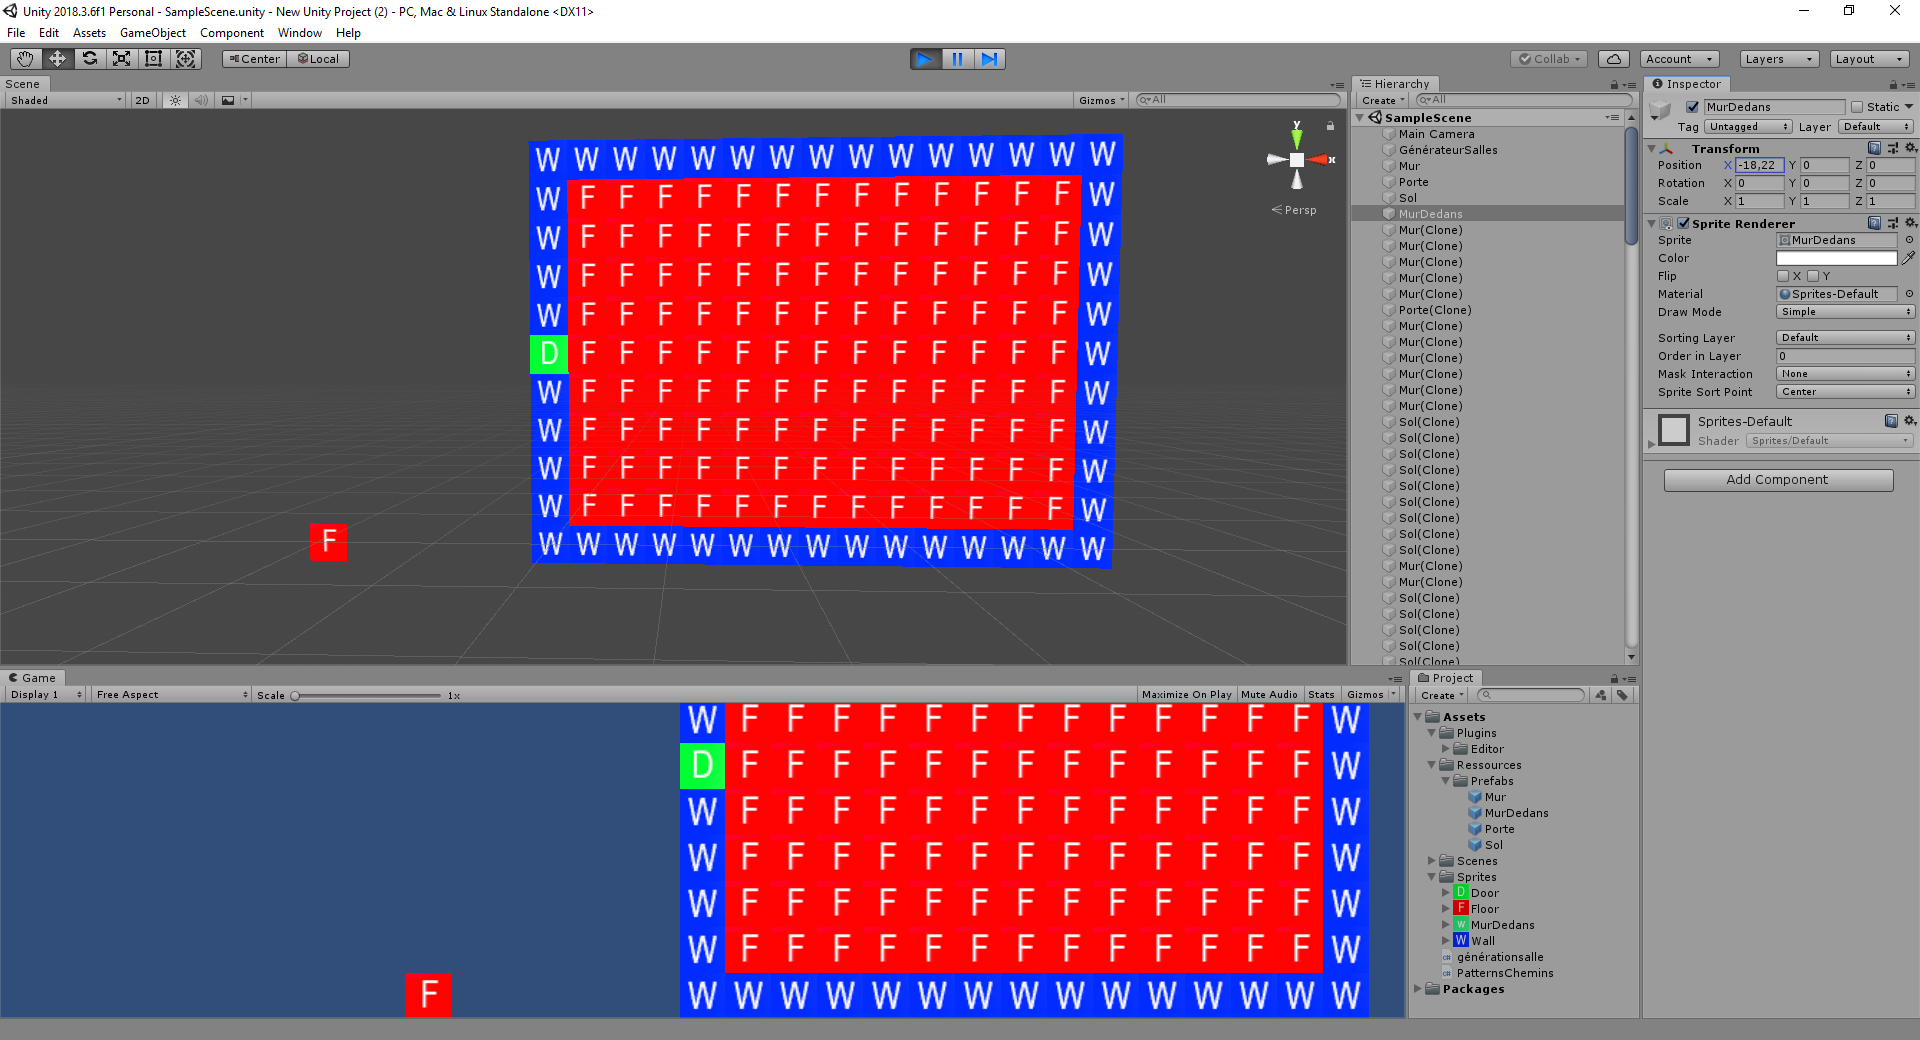
\includegraphics[scale = 0.23]{generation.PNG}
\smallbreak
Figure 8 : Génération d'une salle sans sprites sous Unity
\bigbreak
\bigbreak
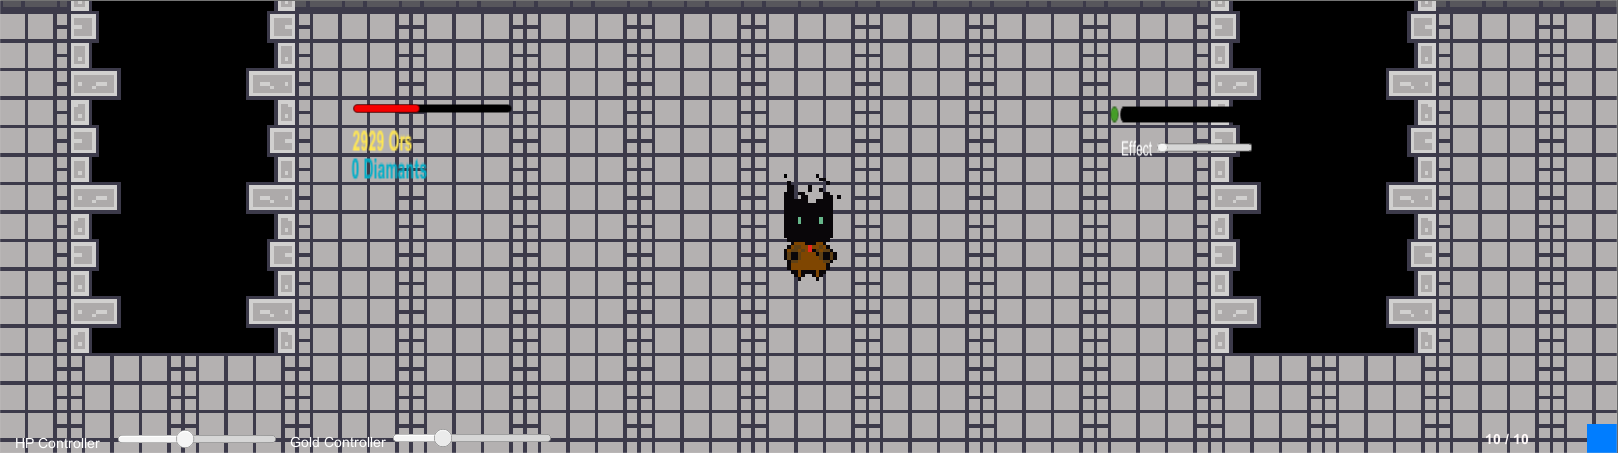
\includegraphics[scale = 0.35]{affichagejeu.PNG}
\smallbreak
Figure 9 : Notre jeu au moment de la soutenance

\end{center}
\end{document}